\documentclass[letterpaper,11pt]{article}
\usepackage[utf8x]{inputenc}
\usepackage{enumerate}
\usepackage{enumitem}
\usepackage{fullpage}
\usepackage{amsmath}

\usepackage{pgf}
\usepackage{tikz}
\usetikzlibrary{arrows,shapes,trees}

%opening
\title{Midterm Exam \\ Classical Mechanics \\ Physics 601 (Fall 2013)}
\date{Due by 9:30am on Thursday October 17, 2013}

\begin{document}

\maketitle

\paragraph*{Instructions}
\begin{itemize}
 \item This midterm exam is governed by William \& Mary Honor Code.
 \item This midterm exam is to be completed \textbf{individually}.
 \item Please carefully explain each step in your answer.
\end{itemize}

\paragraph*{Lagrangian Mechanics}
\begin{enumerate}
 \item Two masses $m_1$ and $m_2$ are connected by a string with fixed length passing through a hole in a smooth table, so that $m_1$ rests on the table and $m_2$ hangs suspended and moves only in the vertical direction.  Consider the motion until $m_1$ reaches the hole.
 \begin{itemize}
  \item Write down the Lagrangian and the equations of motion for this system. Interpret the first integral you encounter.
  \item Under what condition will the hanging mass remain stationary?
  \item Starting from this stationary situation, the mass $m_2$ is pulled down slightly and released again. Investigate the resulting small oscillations in the vertical position of $m_2$.
  \item Calculate the tension in the string for stationary motion using the method of the Lagrange multipliers.
 \end{itemize}
 \item A particle of mass $m$ in a uniform gravitational field is constrained to move on a helical wire with height $z = a\theta$ and radius $r = b$ in cylindrical coordinates.
 \begin{itemize}
  \item Write down the Lagrangian and the equations of motion for this system.
  \item Solve the equations of motion if at $t = 0$ the mass is at $z = 0$.
  \item Find the forces of constraint using the method of the Lagrange multipliers.
 \end{itemize}
 \item A particle of mass $m$ suspended by a massless string of length $\ell$ is stationary in a gravitational field $g$.  It is struck by an impulsive horizontal blow, giving it an initial angular velocity $\omega$.  Introduce a Lagrange multiplier and prove the following statements:
 \begin{itemize}
  \item If $\ell\omega^2 < 2g$, the tension $\tau$ does not vanish and the particle does not reach the horizontal.
  \item If $2g < \ell\omega^2 < 5g$, the particle passes the horizontal and the string becomes slack before the particle comes to rest.
  \item If $5g < \ell\omega^2$, the string always remains taut and the particle executes periodic circular motion.
 \end{itemize}
 Discuss the role of the tension $\tau$ in the string by showing how these results are changed if the string is replaced by a rigid massless rod.
\end{enumerate}

\paragraph*{Hamiltonian Mechanics}
\begin{enumerate}[resume]
 \item Show that the transformation
 \begin{eqnarray*}
  Q & = & p + i \alpha q, \\
  P & = & \frac{1}{2i\alpha}(p-i\alpha q),
 \end{eqnarray*}
 is canonical and find a generating function.  Use this transformation to solve the simple linear harmonic osccilator problem.
 \item A particle moving in one dimension sees a force $F(t) = \lambda t$ that is linearly increasing with time.  Solve the equations of motion using Hamilton's principal function for the initial conditions $x(0) = 0$ and $p(0) = mv_0$.
 \item A particle with mass $m$ is moving in periodic motion in one dimension under the influence of a potential $V(x) = k|x|$.  Use action-angle variables to find the frequency of the motion as a function of the particle energy $E$. [20 points]
 \begin{center}
  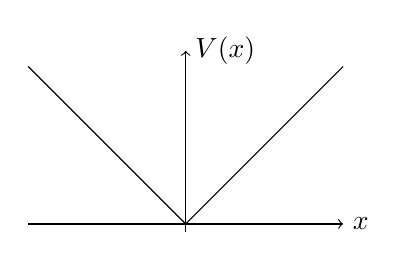
\begin{tikzpicture}
   \draw (-2,0)[->] -- (2,0) node[right] {$x$};
   \draw (0,-0.1)[->] -- (0,2.2) node[right] {$V(x)$};
   \draw (-2,2) -- (0,0) -- (2,2);
  \end{tikzpicture}
 \end{center}
\end{enumerate}

\end{document}
